\scanpage{22}

\diagram{\begin{tikzcd}[ampersand replacement=\&,column sep=small,row sep=small]
\mu_5\arrow[d,dash] \& \& I\unsure{\in|\subset|c} Q\arrow[dl]\\
\mu_5^*\arrow[d,dash] \& \unsure{D_5|D'_5|\mathbb V_5}_{\unsure{S|s}}\arrow[d] \&\\
{} \& S\arrow[u,bend left=44]\arrow[dl] \&\\
\mathbb V_5\arrow[d,dash] \& \&\\
\mathbb Z[\frac14] \& \&
\end{tikzcd}}
\[
 \cos'(D_i,D_j)^2+\cos'(D_i,D_j)
\]
$\cos'(D_i,D_j)$ indépendant de $i,j$ pour $i\ne j$. Soit $c$

$c$

a) $\exists$ des icos. loc. \unsure{ét.quement|étliquement} $\forall c$ donné \unsure{où|i.e.} $\boxed{c^2+c-1=0}$

b) Deux icos. \inserted{\unsure{de|$q$} $=c$} sont loc. conjugués par $SO(Q)$

c) Le groupe d'isotropie d'un icosaèdre \inserted{dans $SO(Q)$} (groupe des autom. d'un icosaèdre) est \inserted{fini} étale $/S$, et ses fibres géom. isom. au gr-pe \uline{alterné} à $5$ \uline{lettres}.

\figure{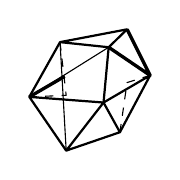
\begin{tikzpicture}[line join=round,scale=.65]
\coordinate (a) at (0,1.05); \coordinate (b) at (.60,2.12); \coordinate (c) at (1.91,2.37); \coordinate (d) at (2.36,1.47); \coordinate (e) at (1.77,.36); \coordinate (f) at (.72,0); \coordinate (g) at (1.45,.94); \coordinate (h) at (1.55,2.02);
\draw[thick] (a)--(b)--(c)--(d)--(e)--(f)--cycle (a)--(g)--(h)--(b) (c)--(h)--(d)--(g)--(f) (e)--(g);
\draw (a)--(h) (b)--(f); \draw[dashed] (b)--(.72,1.08)--(a) (e)--(1.91,1.33)--(d);
\draw[very thick] (c)--(d)--(h) (a)--(.69,1.45);
\end{tikzpicture}}
icosaèdre projectif --- icosaèdre

\figure{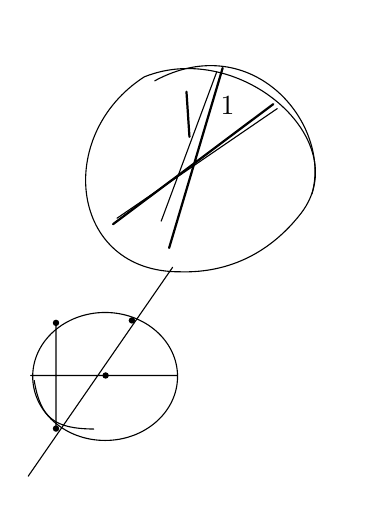
\begin{tikzpicture}[scale=.63,line cap=round]
\draw (.1,1.65) .. controls (-2.13,1.64) and (-2.44,4.41) .. (-.62,5.58) .. controls (1.30,6.35) and (3.66,4.29) .. (2.54,2.83) .. controls (1.95,2.07) and (1.13,1.62) .. (.1,1.65);
\draw (-.41,5.5) .. controls (1.55,6.56) and (3.16,4.64) .. (2.76,3.22);
\draw[thick] (-1.25,2.61)--(1.98,5.03) (-.12,2.13)--(.96,5.76) (.29,4.37)--(.23,5.28);
\draw (-.28,2.67)--(.84,5.68) (-1.17,2.73)--(2.06,4.94); \node at (1.06,5.00) {$1$};
\draw (-1.41,-.46) ellipse (1.46 and 1.29);
\draw (-2.91,-.44)--(.04,-.44) (-2.96,-2.47)--(-.05,1.74) (-2.4,.62)--(-2.4,-1.51);
\draw (-2.84,-.54) .. controls (-2.71,-1.31) and (-2.43,-1.51) .. (-1.64,-1.52);
\foreach \p in {(-2.4,.62),(-.87,.67),(-1.4,-.44),(-2.4,-1.51)}\fill \p circle (.065);
\end{tikzpicture}}
\[
 \begin{gathered}
 1-\unsure{r|\gamma}=r^2\qquad 2-r=1+r^2\\
 r^2+r-1=0\\
 \cos\alpha=\frac{\overset{\cos\alpha}{\deleted{\unsure{a|4}}\,r/2}}{1-r/2}
 =\frac r{2-r}=a+br=\tfrac15(2r+1)=\deleted{\unsure{1/6}}\,\bigl(\tfrac1{\sqrt5}\bigr)
 \end{gathered}
\]
\[
 \begin{aligned}
 \cos2\alpha&=\cos^2\alpha-\sin^2\alpha=2\cos^2\alpha-1=2\frac{r^2}{4-4r+r^2}-1\\
 &=\frac{2(1-r)}{4-4r+1-r}-1\\
 &=\frac{2-2r}{5(1-r)}-1\\
 &=\tfrac25-1=\bigl(-\tfrac35\bigr)\\
 2\cos2\alpha&=-\tfrac65
 \end{aligned}
\]
\[
 \tfrac{2}{25}[4r^2+4r+1]-1\qquad
 \underbrace{4-\deleted{4r}+\deleted{4r}+1}
\]
\[
 \frac{B(x,y)^2}{Q(x)Q(y)}-2=-\tfrac65\ \unsure{2}
 \qquad 2a+(2b-1\inserted{{}-a})r\unsure{-|=|+}br^2=0
\]
\[
 \boxed{B(x,y)^2=\tfrac45 Q(x)Q(y)}
 \qquad r^2+(-2+\tfrac1b+\tfrac ab)r-\tfrac{2a}{b}=0
\]
\[
 -\tfrac{2a}{b}=-1\qquad\boxed{b=2a}\qquad a=\tfrac15\quad b=\tfrac25
\]
\[
 -2+\tfrac{1}{2a}+\tfrac12=1
\]
en car. $2$, \unsure{en effet|cela fait}
\[
 B(x,y)^2=0\qquad \tfrac{1}{2a}=\tfrac52\qquad a=\tfrac15
\]
\[
 \cos'2\alpha=\quad
 2\cos2\alpha=2(2\cos^2\alpha-1)=(2\cos\alpha)^2-2
\]
donc si $2$ \unsure{bon} \deleted{\unsure{alors}} \unsure{si deux}

cela signifie \deleted{$y\perp x$} $y\parallel x$
\[
 \tfrac12 B=B' \qquad \boxed{B'(x,y)^2=\tfrac15 Q(x)Q(y)}
\]
\figure{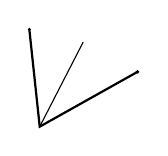
\begin{tikzpicture}[scale=.6]
\draw[thick] (0,2.06)--(.22,0)--(2.29,1.16); \draw (.22,0)--(1.14,1.79);
\fill (0,2.06) circle (.035); \fill (2.29,1.16) circle (.04);
\end{tikzpicture}}
% archive sheet number: 21
